\section{Preliminaries}

\subsection{A Brief Recapitulation of Molecular Featurization Techniques}
\label{sec:featurization-recap}

Molecular featurizations translate chemical information of molecules into representations that can be understood by machine learning algorithms.
Concretely, we consider the following molecular featurizations covering string-, graph-, scalar-, and vector-based representations for 1D/2D molecules and 3D structures, which are popular in literature \cite{Ramsundar:2019dl,Atz:2021hj}:
\begin{itemize}
	\item \textbf{2D topology graphs} model atoms and bonds as nodes and edges respectively. It is arguably a common technique, especially for capturing substructure information by means of graph topology.

	\item \textbf{3D geometry graphs} incorporate atomic coordinates (conformations) in their representations and are able to depict how atoms are positioned relative to each other in the 3D space. We consider conformers in an equilibrium state, corresponding to the minima in a potential energy surface.
	
	\item \textbf{Morgan fingerprints} \cite{Morgan:1965tg,Glem:2006cf} encode molecules in fixed-length binary strings, with bits indicating presence or absence of specific substructures.
	They represent each atom according to a set of atomic invariants and iteratively update these features among neighboring atoms using a hash function.
	
	\item \textbf{SMILES strings} are a concise technique that represents chemical structures in a linear notation using ASCII characters, with explicitly depicting information about atoms, bonds, rings, connectivity, aromaticity, and stereochemistry.
\end{itemize}

\subsection{Learning Representations with Different Featurizations}

Next, we introduce four encoders with different inductive bias to capture the intrinsic information with each featurization.
Here we only discuss the high-level design of each encoder; please refer to \cref{supp:view-encoders} for detailed implementations of each encoder.

\paragraph{Notations.}
Each molecule can be represented as an undirected graph, where nodes are atoms and edges describe inter-atomic bonds.
Formally, each graph is denoted as \(\mathcal{G} = (\bm{A}, \bm{R}, \bm{X}, \tens{E})\), where \(\bm{A} \in \{0,1\}^{N\times N}\) is the adjacency matrix of \(N\) nodes, \(\bm{R} \in \mathbb{R}^{N \times 3}\) is the 3D position matrix, \(\bm{X} \in \mathbb{R}^{N \times K}\) is the matrix of atom attributes of \(K\) dimension, and \(\tens{E} \in \mathbb{R}^{N \times N \times E}\) is the tensor for bond attributes of \(E\) dimension.
Additionally, each molecule is attached with a binary fingerprint vector \(\bm{f} \in \{0, 1\}^{F}\) of length \(F\) and a SMILES string \(\mathbf{S} = [s_j]_{j=1}^{S}\) of length \(S\).
In what follows, the subscript \(i\) is used to index the \(i\)-th molecule.

\paragraph{Embedding 2D graphs.}
To capture the 2D topological information, we employ a widely-used Graph Isomorphism Network (GIN) model \cite{Xu:2019ty} denoted by \(f_\text{2D}\), which receives as input the graph adjacency matrix and attributes of atoms and bonds, and produces the embedding vector \(\bm{z}^\text{2D}_i \in \mathbb{R}^{D}\):
\begin{equation}
	\bm{z}^\text{2D}_i = f_\text{2D}(\bm{X}_i, \tens{E}_i, \bm{A}_i).
\end{equation}

\paragraph{Embedding 3D graphs.}
To model additional spatial coordinates associated with atoms, we leverage SchNet \cite{Schutt:2017wh} as the backbone, which models message passing as continuous-filter convolutions and is able to preserve rotational invariance for energy predictions.
We denote its encoding function as \(f_\text{3D}\) which takes atom features and positions as input and produces the 3D embedding \(\bm{z}^\text{3D}_i \in \mathbb{R}^{D}\):
\begin{equation}
	\bm{z}^\text{3D}_i = f_\text{3D}(\bm{X}_i, \bm{R}_i).
\end{equation}

\paragraph{Embedding molecular fingerprints.}
Since there is a lack of proper neural encoders for fingerprints, we propose an attention-based network to model interactions of feature fields in fingerprint vectors, which considers the discrete and extremely sparse nature of fingerprints.
Specifically, we first transform all \(F\) feature fields into a dense embedding matrix \(\bm{F}_i \in \mathbb{R}^{F \times D_\text{F}}\) via embedding lookup.
Then, we use a multihead self-attention network \(f_\text{FP}\) \cite{Vaswani:2017ul} to model the interaction among those feature fields, resulting in an embedding matrix \(\widehat{\bm{Z}}^\text{FP}_i \in \mathbb{R}^{F \times D_\text{F}}\).
Following that, we perform sum pooling and use a linear model \(f_\text{LIN}\) to obtain the final fingerprint embedding \(z^\text{FP}_i \in \mathbb{R}^{D}\):
\begin{equation}
	\widehat{\bm{Z}}^\text{FP}_i = f_\text{FP}(\bm{F}_i), \qquad\qquad\qquad \bm{z}^\text{FP}_i = f_\text{LIN} \left(\sum_{d=1}^{D_\text{F}} \widehat{\bm{Z}}^\text{FP}_{i,d}\right).
\end{equation}

\paragraph{Embedding SMILES strings.}

To encode SMILES strings, we use a pretrained RoBERTa \cite{Liu:2019dd} as the backbone model.
As SMILES strings do not possess consecutive relationships, the RoBERTa model is pretrained using the masked language model as the only objective, unlike conventional natural language models \cite{Devlin:2019uk}.
After that, in order to reduce the computational burden, we freeze the RoBERTa encoder (denoted by \(f_\text{SM}\)) in our model and employ an additional learnable MultiLayer Perceptron (MLP) on the representation \(\bm{s}_i \in \mathbb{R}^{D_\text{S}}\) to get the final embedding \(\bm{z}^\text{SM}_i \in \mathbb{R}^{D}\):
\begin{equation}
	\bm{s}_i = f_\text{SM}(\mathbf{S}_i), \qquad\qquad\qquad \bm{z}^\text{SM}_i = f_\text{MLP}(\bm{s}_i).
\end{equation}

\subsection{Case Studies}


	\setlength{\intextsep}{3pt}
\begin{wrapfigure}{r}{0.4\textwidth}
	\centering
	\captionof{figure}{(a) Chirality: even if two graphs are isomorphic, they can have two distinct stereochemistry structures. (b) The aromatic ring is an important functional group.}
	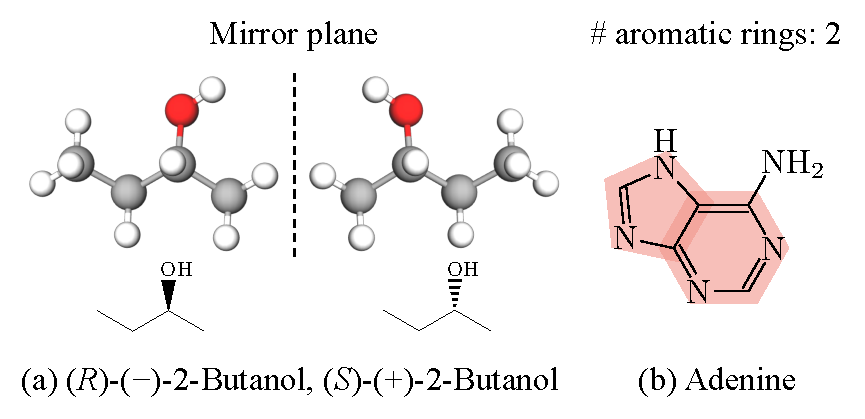
\includegraphics[width=\linewidth,bb=0 0 415 201]{figures/case-study.pdf}
\end{wrapfigure}
In this section, we present two case studies---chirality classification and aromatic ring counting---to demonstrate that the representation ability of each featurization with the corresponding neural encoder is different.
For chirality classification, we randomly select 10K molecules with one chirality center from GEOM-Drugs \cite{Axelrod:2022da} and test whether the representations obtained using the four featurizations can classify tetrahedral chiral centers as R/S.
For aromatic ring counting, we randomly draw another 10K molecules and test whether these models can recognize the number of aromatic rings of each molecule.
Note that both chirality properties and ring counts are informative chemical descriptors \cite{Ritchie:2009ti} and can be easily computed with existing implementations such as RDKit \cite{Landrum:2022rd}.

\begin{wraptable}{r}{0.4\textwidth}
	\captionof{table}{Results of two case studies with different featurizations: chirality classification and aromatic ring count regression.}
	\begin{tabular}{ccccc}
	\toprule
	Target & 2D & 3D & SM & FP \\
	\midrule
	Chirality (AP, \(\uparrow\)) &   0.4952    &    0.4959   &    \textbf{0.5505}   & 0.5246 \\
	\#Rings (MAE, \(\downarrow\)) &   \textbf{0.1949}    &   0.2021    &   0.3077    & 0.2590 \\
	\bottomrule
	\end{tabular}
	\label{tab:case-studies}
\end{wraptable}
We report classification and regression performance in Average Precision (AP) and Mean Absolute Error (MAE) respectively. The results are summarized in \cref{tab:case-studies}. 
It is seen from the table that no single featurization performs the best on all targets and four representations contain complementary information to each other, suggesting us to leverage multiple featurizations for molecular pretraining.
